


                                                                                                  %%%%       GRAPHS           %%%

\chapter {Graphs}
vertices or nodes, edges (directed or undirected), head, tail, in-degree, out-degree, self-loop (reflexive), was covered in the chapter on functions.
Famous algorithms for graph traversal


\section {Graphs and Graph Models}
\begin{definition}[Graph]\index{graph}\index{vertex}\index{edge}
A \textit{graph} $G =(V,E)$ consistes of a non-empty set $V$ of \textit{vertices} or \textit{nodes} and $E$, a set of \textit{edges}. Each edge has either one or two vertices associated ith it, called its \textit{endpoints}. An edge is said to \textit{connect} its endpoints.
\end{definition}
\begin{notes}
The number of vertices does not need to be finite. But we will only discuss finite graphs in this outline.
\end{notes}

\begin {definition} [Simple Graph]\index{simple graph}
A graph in which each edge connects two different vertices and where no two edges connect the same pair of vertices is called a \textbf{simple graph}. The edge in a simple graph can be denoted by the set of vertices it connects.
\end{definition}

\begin {definition}[Multigraph]\index{multigraph}
Graphs that have multiple edges connecting the same vertices are called \textbf{multigraphs}. We say that each edge has a multiplicity of edges between the two vertices.
\end{definition}

\begin{definition}[Directed or Digraph]\index{directed graph}\index{digraph}
A \textit{directed graph} (or \textit{digraph} $(V,E)$ consists of a nonempty set of vertices $V$ and a set of \textit{directed edges} or \textit{arcs} $E$. Each directed edge is associated with an ordereed pair of vertices. The directed edge associated with the ordered pair $(u,v)$ is said to start with $u$ and end at $v$. When presented in a picture, the directed edge has an arrow that starts at the vertex $u$ and ends at $v$. A directed graph may also have multiple directed edges.
\end{definition}

Graphs model a great many applications in software engineering. They include Acuaintanceship Graphs, Influence Graphs, The Hollywood Graph, Round-Robin Tournaments, Collaboration Graphs, Road Maps, Call Graphs, and the WWW.

\section {Graph Terminology and Special Types of Graphs}
\begin{definition}[Edges in an Undirected Graph]
Two vertices $u$ and $v$ in an undirected graph $G$ are called \textit{adjacent} (or \textit{neighbors} in $G$ if $u$ and $v$ are endpoints of an edge of $G$. If $e$ is associated with $\{u,v\}$, the edge $e$ is called \textit{incident with} the vertices $u$ and $v$. The edge $e$ is also said to \textit{connect u} and \textit{v}. The vertices $u$ and $v$ ar called \textit{endpoints} of an edge associated with $\{u,v\}$.
\end{definition}

\begin{definition}
The \textit{degree of a vertex in an undirected graph} is the number of edges incident with it, except that a loop at a vertex contributes twice to the degree of that vertex. The degree of the vertex $v$ is denoted by deg($v$). A vertex of degree zero is called \textbf{isolated} while a vertex with degree one is called \textbf{pendant}
\end{definition}

\begin{theorem} [The Handshaking Theorem]\index{handshaking theorem}
Let $G=(V,E)$ be an undirected graph with $e$ edges. Then 
$$2e = \Sigma_{v\in V} deg(v)$$.
\end{theorem}
\begin{notes}
This is true even when multiple edges and loops are present.
\end{notes}

\begin{theorem}
An undirected graph has an even number of vertices of odd degree.
\end{theorem}

\begin{definition}
When $(u,v)$ is an edge of the graph $G$ with directed edges, $u$ is said to be \textit{adjacent to v} and $v$ is said to be \textit{adjacent from u}. The vertex $u$ is called the \textit{initial vertex} of $(u,v)$, and $v$ is called the \textit{terminal} or \textit{end vertex} of $(u,v)$. The initial and terminal vertex of a loop are the same.
\end{definition}

\begin{definition}
In a graph with directed edges, the \textit{in-degree of a vertex v}, denoted by $\text{deg}^-(v)$, is the number of edges with $v$ as their terminal vertex. The \textit{out-degree of v}, denoted by $\text{deg}^+(v)$, is the number of edges with $v$ as their initial vertex. (Note that a loop at a vertex constributes 1 to both the in-degree and the out-degree of this vertex.)
\end{definition}

\begin{theorem}
Let $G=(V,E)$ be a graph with directed edges. Then
$$\Sigma_{v\in V} \text{deg}^-(v) = \Sigma_{v \in V} \text{deg}^+(v) = \lvert E \rvert$$
\end{theorem}

\begin{definition}Here are the definitions of some common simple graphs:\\
A \textbf{Complete Graph on $n$-vertices} is a simple graph that contains exactly one edge between each pair of distinct vertices. It is denoted by $K_n$.\\
A \textbf{Cycle} of $n$ vertices, $n\ge3$, $v_1,v_2, \dots ,v_3$ has edges $\{v_1,v_2\},\{v_2,v_3\}, \dots ,\{v_{n-1},v_n\}, \{v_n,v_1\}$. It is denoted $C_n$.\\
A \textbf{Wheel} is created by taking a cycle, $C_n$, adding a single vertex $v$ and adding an edge from the new vertex $v$ to each of the $n$ existing vertices of the cycle. It is designated $W_n$.\\
The \textbf{$n$-dimensional hypercube} or \textbf{$n$-cube} is the graph that has vertices representing the $2^n$ bit strings of length ....blah blah
\end{definition}

\begin{definition}[Bipartite Graph]\index{bipartite graph}
A simple graph $G$ is called \textit{bipartite} if its vertex set $v$ can be partititoned into two disjoint sets $V_1$ and $V_2$ such that evry edge in the graph connects a vertex in $V_1$ and a vertex in $V_2$. For such a graph we call the pair $(V_1,V_2) $ a \textit{bipartition} set $V$ of $G$.
\end {definition}

\begin{theorem}
A simple graph is bipartte if an donly if it is possible to assign one of two different colors to each vertex of the graph so that no two adjacent vertices are assigned the same color. This is called a \textit{graph coloring}.
\end{theorem}

\begin{definition}[Complete Bipartite Graphs]
The \textbf{complete bipartite graph $K_{m,n}$} is the graph that has its vertex set partitioned into two subsets of $m$ and $n$  vertices, respectively. There is an edge between two vertices if and only if one vertex is in the first subset and the other vertex is in the second subset. 
\end{definition}

\begin{definition}
A \textit{subgraph of a graph} $G=(V,E)$ is a graph $H=(W,F)$, where $ W \subset V$ and $F \subset E$. A subgraph $H$ of $G$ is a \textit{proper subgraph} of $G$ if $H \neq G$.
\end{definition}

\begin{definition}
The \textit{union} of two simple graphs $G_1 = (V_1,E_1)$ and $G_2=(V_2,E_2)$ is the simple graph with vertext set $V_1 \cup V_2$ and edge set $E_1 \cup E_2$. The unions of $G_1$ and $G_2$ is denoted by $G_1 \cup G_2$.
\end{definition}


\section {Representing Graphs and Graph Isomorphism}
Sometimes we look at graphics that depict two different graphs but we see that while they look different we can make one match to the other by moving vertices around. This leads us to look at how we represent graphs and to define what we mean by saying two graphs are somehow the same.

There are two common way that graphs are represented using tables and these are useful in software engineering. We look at adjacency lists and adjacency matrices.

\begin{definition}
A simple graph $G$ can be represented by listing each vertex and the vertices that are adjacent to it. This is called an \textbf{adjacency list}. This can be extended to include a representation of directed graphs. Note that the size of the lists will be half the size of an undirected graph.
\end{definition}

\begin{definition}
A simple graph $G$ can be represented by a two dimensional matrix with the vertices of the graph on both axes. The presence of an edge between them can be represented by a value in the matrix. 

Suppose that $G=(V,E)$ is a simple graph where $\lvert V \rvert = n$. Suppose that the vertices of $G$ are listing arbitraryily as $v_1,v_2, \dots ,v_n$. The \textbf{adjacency matrix $A$} (or $A_G$) of $G$, with respect to this listing of the vertices, is the $n \times n$ zero-one matrix with 1 as its $(i,j)$th entry when $v_i$ and $v_j$ are adjacent, and 0 as its $(i,j)$th entry when they are not adjacnt. In other words, if its adacency matrix is $A=[a_{ij}]$, then 

cases

\end{definition}

\begin{definition}
Graphs can be represented by an \textbf{incidence matrix}. Let $G=(V,E)$ be an undirected graph. Suppose that $v_1,v_2, \dots ,v_n$ are the vertices and $e_1,e_2, \dots ,e_m$ are the edges of $G$. Then the incidence matrix with respect to this ordering of $V$ and $E$ is the $n \times n$ matrix $M=[i,j]$, where

cases
\end{definition}

\begin{definition}
The simple graphs $G_1=(V_1,E_1)$ and $G_2=(V_2,E_2)$ are \textit{isomorphic} if there is a one-to-one and onto function (a bijection) $f$ from $V_1$ to $V_2$ with the property that $a$ and $b$ are adjacent in $G_1$ if and only if $f(a)$ and $f(b)$ are adjacent in $G_2$, for all $a$ and $b$ in $V_1$. Such a function $f$ is called an \textit{isomorphism}.
\end{definition}

Worst case algorithms to determine graph isomorphism have exponential worst case time complexity. However there are algorithms that have linear average time complexity for graph isomorphism. 

\section {Connectivity}


\section {Euler Paths and Circuits}
  \begin{figure}[htbp]
   \centering
   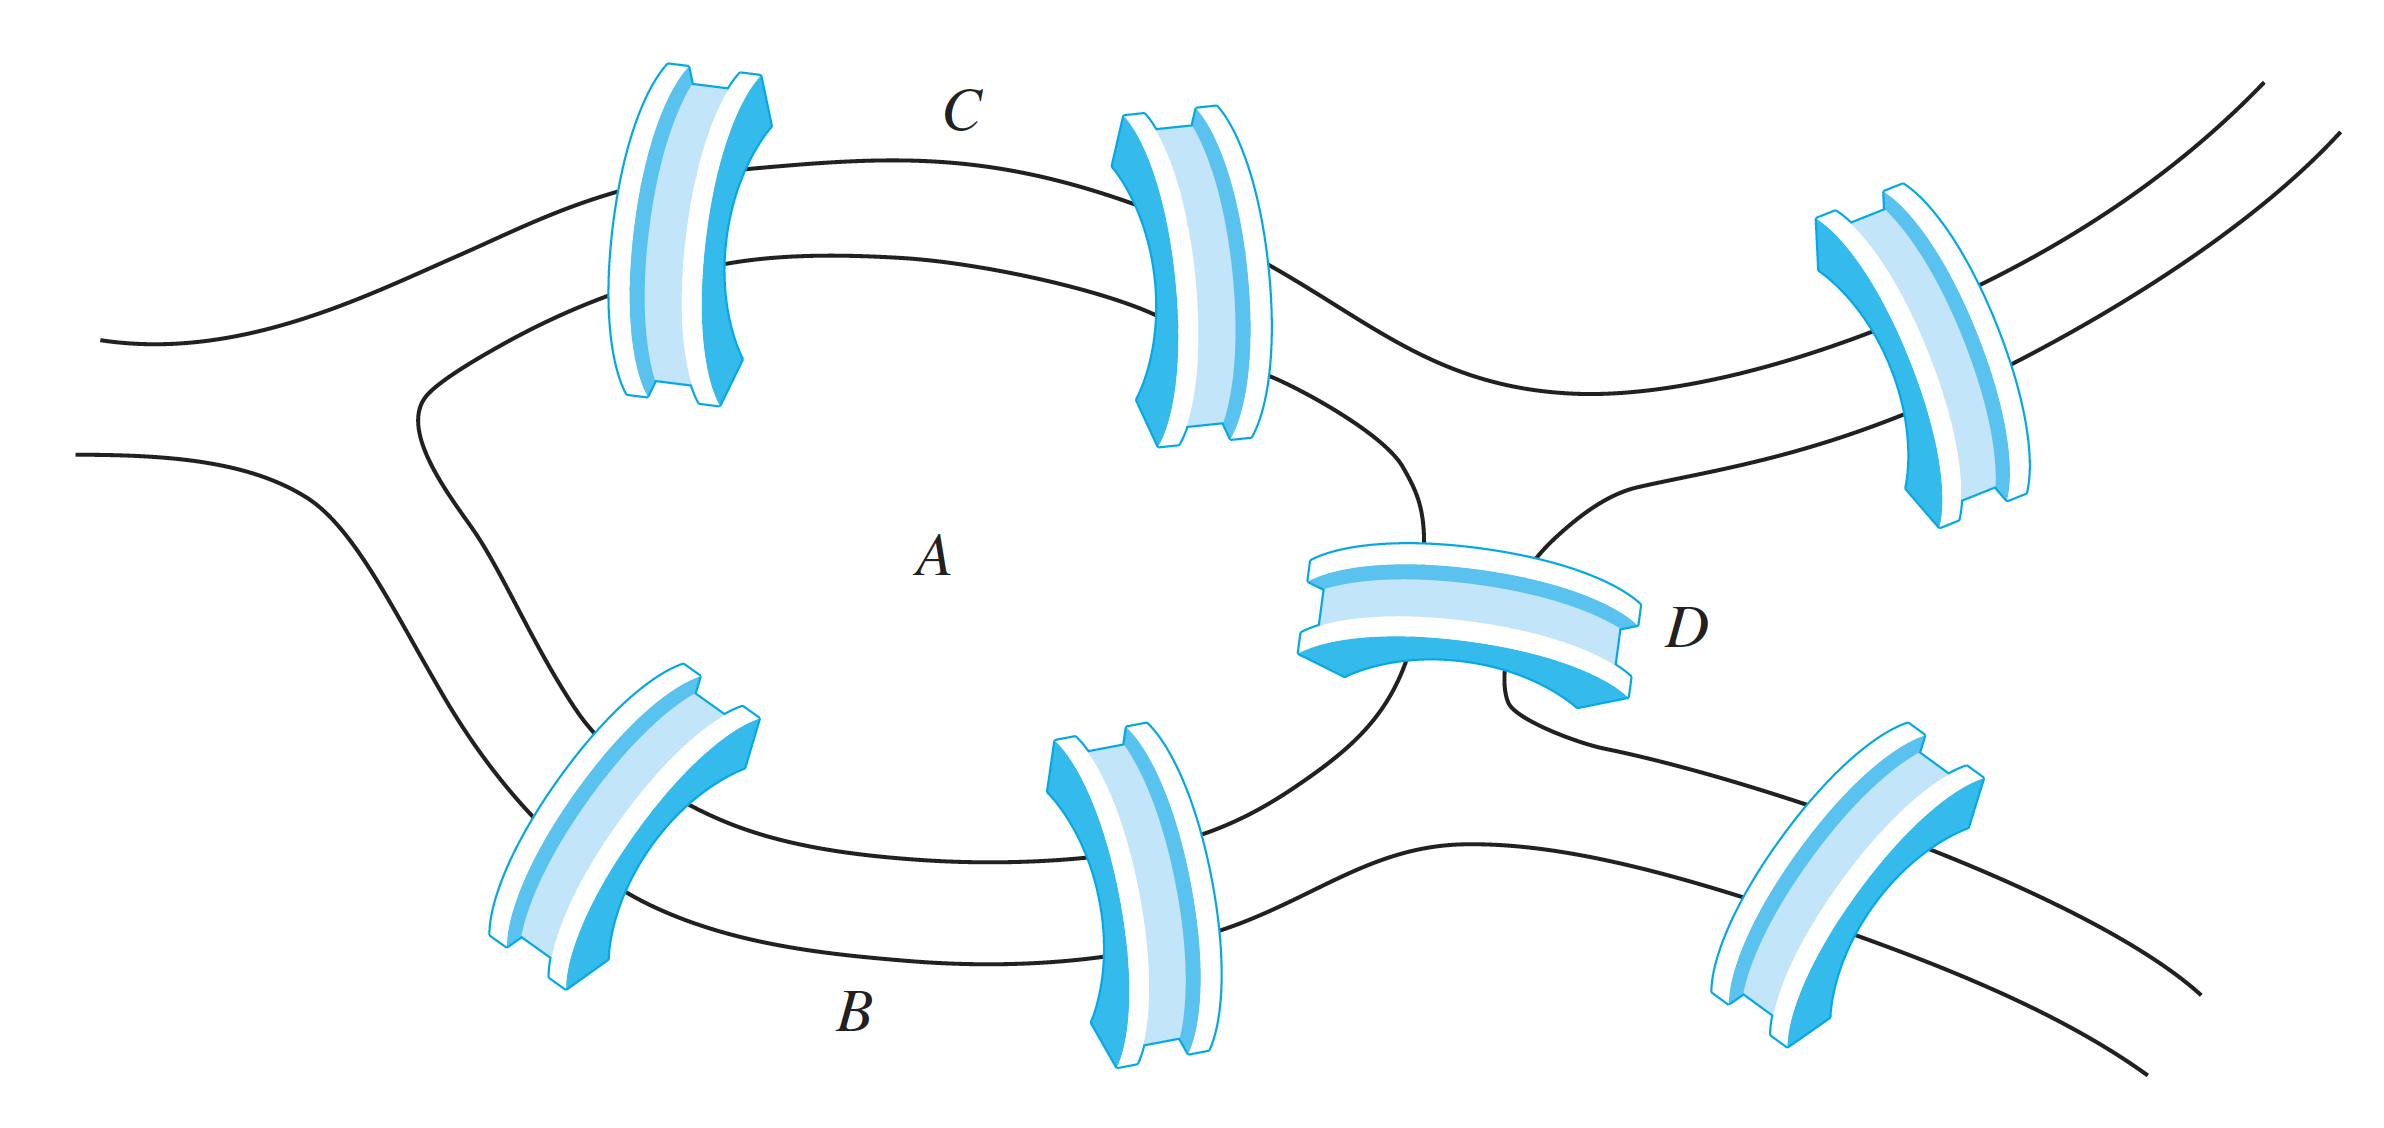
\includegraphics [width=5in]{Figure-10-6-1-BridgesOfKoenigsberg}
%figure from Rosen
   \caption{The Bridges of Koenigsberg}
   \label{figure:BridgesOfKoenigsberg}
\end{figure}

\begin{definition}
An \textit{Euler circuit} in a graph $G$ is a simple circuit containing every edge of $G$. An \textit{Euler path} in $G$ is a simple path containing every edge of $G$.
\end{definition}

\begin{theorem}
A connected multigraph with at least two vertices has an Euler curcuit if and only if each of its vertices has even degree.
\end{theorem}

NECESSARY AND SUFFICIENT CONDITIONS FOR EULER CIRCUITS AND PATHS
There are simple criteria for determining whether a multigraph has an Euler circuit or an Euler
path. Euler discovered them when he solved the famous Königsberg bridge problem. We will
assume that all graphs discussed in this section have a finite number of vertices and edges.
What can we say if a connected multigraph has an Euler circuit? What we can show is that
every vertex must have even degree. To do this, first note that an Euler circuit begins with a
vertex a and continues with an edge incident with a, say {a, b}. The edge {a, b} contributes one
to deg(a). Each time the circuit passes through a vertex it contributes two to the vertex’s degree,
because the circuit enters via an edge incident with this vertex and leaves via another such edge.
Finally, the circuit terminates where it started, contributing one to deg(a). Therefore, deg(a)
must be even, because the circuit contributes one when it begins, one when it ends, and two
every time it passes through a (if it ever does). A vertex other than a has even degree because
the circuit contributes two to its degree each time it passes through the vertex.We conclude that
if a connected graph has an Euler circuit, then every vertex must have even degree.
Is this necessary condition for the existence of an Euler circuit also sufficient? That is, must
an Euler circuit exist in a connected multigraph if all vertices have even degree? This question
can be settled affirmatively with a construction.

Algorithm: Constructing Euler Circuits

\begin{theorem}
A connected multigraph has an Euler path but not an Euler circuit if and only if it has exactly two vertices of odd degree.
\end{theorem}
\section{Hamilton Paths and Circuits}
\begin{definition}
A simple path in a graph $G$ that passes through every vertex exactly once is called a \textit{Hamilton path}, and a simple circuit in graph $G$ that passes through everty vertex exactly once is called a \textit{Hamilton circuit}. That is, the simple path $x_0,x_1,\dots ,x_{n-1},x_n$ and $x_i\neq x_j$ for $0 \le i  < j \le n$, and the simple circuit $x_0,x_1, \dots ,x_{n-1},x_n,x_0$ (with $n>0$) is a Hamilton circuit if $x_0,x_1, \dots x_{n-1},x_n$ is a Hamilton path.
\end{definition}
CONDITIONS FORTHE EXISTENCE OF HAMILTON CIRCUITS Is there a simple way
to determine whether a graph has a Hamilton circuit or path? At first, it might seem that there
should be an easy way to determine this, because there is a simple way to answer the similar
question of whether a graph has an Euler circuit. Surprisingly, there are no known simple
necessary and sufficient criteria for the existence of Hamilton circuits. However, many theorems
are known that give sufficient conditions for the existence of Hamilton circuits. Also, certain
properties can be used to show that a graph has no Hamilton circuit. For instance, a graph with a
vertex of degree one cannot have a Hamilton circuit, because in a Hamilton circuit, each vertex
is incident with two edges in the circuit. Moreover, if a vertex in the graph has degree two, then
both edges that are incident with this vertex must be part of any Hamilton circuit. Also, note
that when a Hamilton circuit is being constructed and this circuit has passed through a vertex,
then all remaining edges incident with this vertex, other than the two used in the circuit, can be
removed from consideration. Furthermore, a Hamilton circuit cannot contain a smaller circuit
within it.

\begin{theorem}[Dirac's Theorem]
If $G$ is a simple graph with $n$ vertices with $n \ge 3$ such that the degree of every vertex in $G$ is at least $\frac{n}{2}$, then $G$ has a Hamilton circuit.
\end{theorem}

\begin{theorem}[Ore's Theorem]
If $G$ is a simple graph with $n$ vertices with $n \ge 3$ such that deg($u$)+deg($v$) $\ge n$ for every pair of nonadjacent vertices $u$ and $v$ in $G$, then $G$ has a Hamilton circuit.
\end{theorem}

\section {Shortest Path Problem}
Dijkstra's Algorithm

\begin{theorem}
Dijkstra's algorithm finds the length of a shortest path between two vertices in a connected simple undirected weighted graph.
\end{theorem}

\begin{theorem}
Dijkstra's algorithm uses $O(n^2)$ operations (additions and comparisons) to find the length of a shortest path between two vertices in a connected siple undirected weighted graph with $n$ vertices.
\end{theorem}

\begin{figure}[htbp]
   \centering
   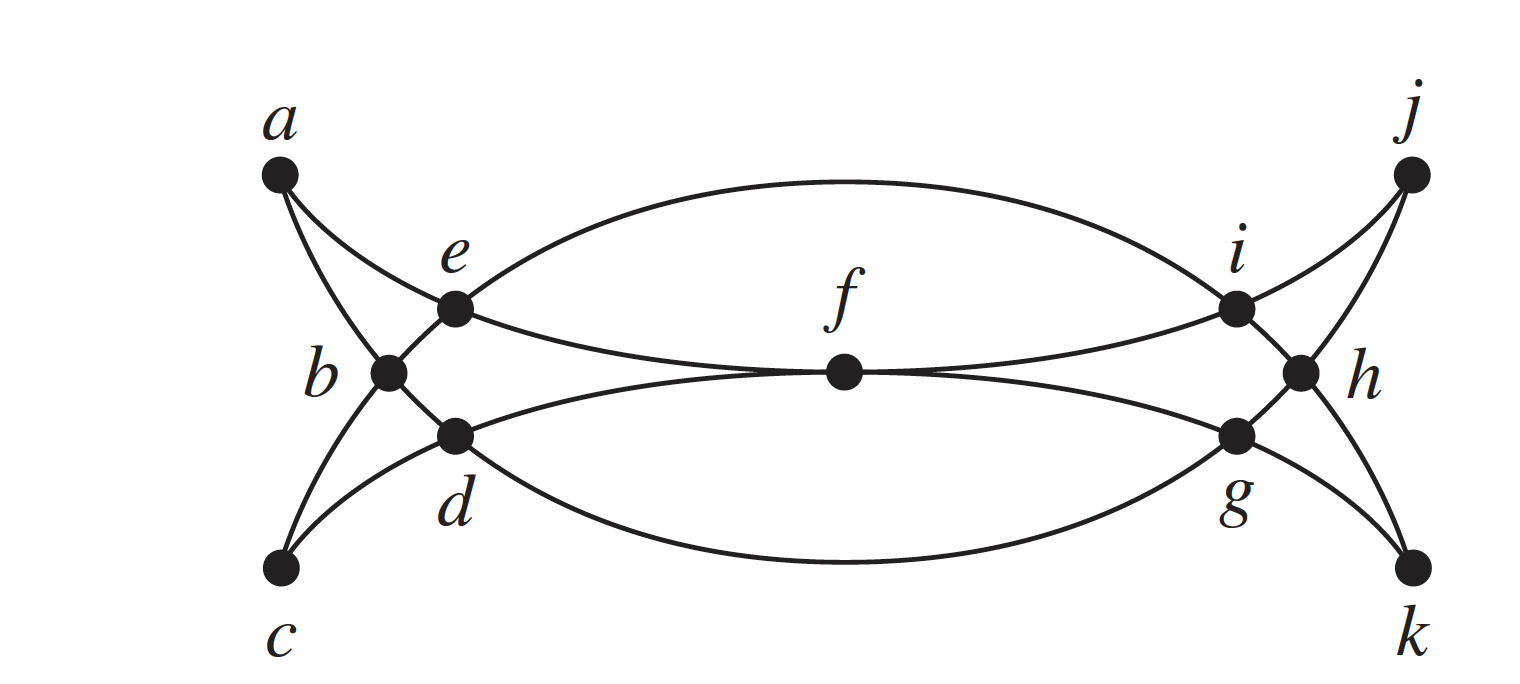
\includegraphics [width=3in]{Figure-10-5-6-MohammedsScimitar}
   \caption{Mohammeds Scimitar}
   \label{figure:Figure-10-5-6-MohammedsScimitar}
\end{figure}

\section {Planar Graphs}
\begin{definition}
A graph is called \textit{planar} if it can be drawn in the plane without any edges crossing (where a crossing of edges is the intersection of the lines or arcs represening them at a point other than their common endpoint). Such a drawing is called a \textit{planar representation} of the graph.
\end{definition}

\begin{theorem}[Euler's Formula]
Let $G$ be a connected planar simple graph with $e$ edges and $v$ vertices. Let $r$ be the number of regions in a planar representation of $G$. Then $r-e-v+2$.
\end{theorem}

\begin{corollary}
If $G$ is a connected planar simple graph with $e$ edges and $v$ vertices, where $v \ge 3$, then $e \le 3v -  6$
\end{corollary}

\begin{corollary}
If $G$ is a connected planar simple, graph then $G$ has a vertex of degree not exceeding five.
\end{corollary}

\begin{corollary}
If a connected planar simple graph has $e$edges and $v$ vertices with $v \ge 3$ and no circuits of length three, then $e \le 2v - 4$.
\end{corollary}

\begin{theorem}
A graph is nonplanar if and only if it contains a subgraph homeomorphic to $K_{3,3}$ or $K_5$.
\end{theorem}

\section {Graph Coloring}
\begin{definition}
A \textit{coloring} of a simple graph is the assignment of  acolor to each vertex of the graph so that no two adjacent vertices are assigned the same color.
\end{definition}

\begin{definition}
The \textit{chromatic number} of a graph is the least number of colors needed for a coloring of this graph. The chromatic number of a graph $G$ is denoted by $\chi(G)$ (where $\chi$ is the Greek letter chi).
\end{definition}

\begin{theorem}[The Four Color Theorem]
The chromatic number of a planar graph is no greater than four.
\end{theorem}

\newpage